%% =======================================================
%% Actividad 13: Construcción de un MiniModelo Preventivo
%%
%% Compilar desde actividades/: ./compilar.sh act13
%% Las figuras de img/ se generan con: python act13.py
%% =======================================================

%% ---- CONFIGURACIÓN ------------------------

\documentclass[11pt,letterpaper]{article}

\usepackage[indice]{tecnm}
\usepackage[T1]{fontenc}
\usepackage{amsmath}
\usepackage{xcolor}
\usepackage[most]{tcolorbox} % Carga tcolorbox con soporte para listings y saltos de página
\tcbuselibrary{listings, skins, breakable}
\setlength{\emergencystretch}{3em} % Evita líneas desbordadas por palabras en \texttt

% Paleta de colores (estilo GitHub Light / VS Code)
\definecolor{codebg}{HTML}{F8F9FA}       % Fondo del código
\definecolor{codehead}{HTML}{E9ECEF}     % Fondo de la barra de título
\definecolor{codeborder}{HTML}{CED4DA}   % Borde de la tarjeta
\definecolor{codetitle}{HTML}{212529}    % Texto del título
\definecolor{codekw}{HTML}{0550AE}       % Palabras clave (import, def, for...)
\definecolor{codefunc}{HTML}{8250DF}     % Funciones y métodos (describe, groupby...)
\definecolor{codestr}{HTML}{0A3069}      % Strings
\definecolor{codecomm}{HTML}{6E7781}     % Comentarios
\definecolor{codenum}{HTML}{8C959F}      % Números de línea
\definecolor{codeid}{HTML}{24292F}       % Texto general

% Configuración base de listings
\lstdefinestyle{pythonestilo}{
  language=Python,
  basicstyle=\ttfamily\footnotesize\color{codeid},
  keywordstyle=\color{codekw}\bfseries,
  keywordstyle=[2]\color{codefunc}, % Estilo secundario para métodos de datos
  stringstyle=\color{teal!80!black},
  commentstyle=\color{codecomm}\itshape,
  morekeywords={as, True, False, None, with, yield, lambda},
  morekeywords=[2]{print, len, sum, max, DataFrame, Series, value_counts, reindex, mean, std, var, randint, normal, seed, cumsum, poisson, binom, pmf, norm, fit, kde, bincount, linspace, train_test_split, make_blobs, GaussianNB, chisquare, pdf, cdf, hist, bar, plot, axhline, axvline, fill_between, subplots, figure, concat, nunique, load_iris, diff, sort, unique},
  numbers=left,
  numberstyle=\tiny\ttfamily\color{codenum},
  stepnumber=1,
  numbersep=10pt,
  showstringspaces=false,
  morestring=[b]{"""},
  tabsize=4,
  breaklines=true,
  breakatwhitespace=true,
  columns=flexible,
  keepspaces=true,
  literate=
    {á}{{\'a}}1 {é}{{\'e}}1 {í}{{\'i}}1 {ó}{{\'o}}1 {ú}{{\'u}}1
    {Á}{{\'A}}1 {É}{{\'E}}1 {Í}{{\'I}}1 {Ó}{{\'O}}1 {Ú}{{\'U}}1
    {ñ}{{\~n}}1 {Ñ}{{\~N}}1 {¿}{{?`}}1 {¡}{{!`}}1 {°}{{$^\circ$}}1
}

% Definición del entorno personalizado \begin{codigo}{Título}{etiqueta}
% \newtcblisting[auto counter, number within=section]{codigo}[2][]{
\newtcblisting[auto counter]{codigo}[2][]{
  listing only,
  breakable,                    % Permite que el bloque se divida si pasa de página
  enhanced,
  colback=codebg,
  colframe=codeborder,
  colbacktitle=codehead,
  coltitle=codetitle,
  fonttitle=\bfseries\small\sffamily,
  boxrule=0.6pt,
  arc=4pt,                      % Bordes redondeados
  left=20pt,                    % Espacio izquierdo para los números de línea
  right=8pt,
  top=6pt,
  bottom=6pt,
  toptitle=4pt,
  bottomtitle=4pt,
  before skip=12pt,
  after skip=12pt,
  listing options={style=pythonestilo},
  title={Código \thetcbcounter: #2},
  #1
}

% Paleta para salida de consola (estilo terminal limpia)
\definecolor{termbg}{HTML}{212529}      % Fondo oscuro tipo terminal
\definecolor{termhead}{HTML}{343A40}    % Barra superior
\definecolor{termtext}{HTML}{F8F9FA}    % Texto claro de alta legibilidad
\definecolor{termborder}{HTML}{495057}  % Borde

% Entorno \begin{consola}[label=out:iris]{Título}
\newtcblisting[auto counter]{consola}[2][]{
  listing only,
  breakable,
  colback=termbg,
  colframe=termborder,
  colbacktitle=termhead,
  coltitle=termtext,
  colupper=termtext,
  fonttitle=\bfseries\small\sffamily,
  boxrule=0.6pt,
  arc=4pt,
  left=8pt,
  right=8pt,
  top=6pt,
  bottom=6pt,
  toptitle=4pt,
  bottomtitle=4pt,
  before skip=12pt,
  after skip=12pt,
  listing options={
    basicstyle=\ttfamily\scriptsize\color{termtext}, % \scriptsize evita que las tablas de Pandas se partan de línea
    breaklines=true,
    columns=fixed,        % Mantiene alineadas las columnas de Pandas
    keepspaces=true,
    showstringspaces=false,
    literate=
      {á}{{\'a}}1 {é}{{\'e}}1 {í}{{\'i}}1 {ó}{{\'o}}1 {ú}{{\'u}}1
      {Á}{{\'A}}1 {É}{{\'E}}1 {Í}{{\'I}}1 {Ó}{{\'O}}1 {Ú}{{\'U}}1
      {ñ}{{\~n}}1 {Ñ}{{\~N}}1 {°}{{$^\circ$}}1
  },
  title={Salida \thetcbcounter: #2},
  #1
}

%% ---- DATOS DE LA MATERIA ------------------------

\materia{Modelos Estadísticos para el Aprendizaje \\ Automático y Ciencia de Datos}
\actividad{Tema 2.3 Distribuciones como Base para Modelos Predictivos Bayesianos \\ Actividad 13 - Construcción de un MiniModelo Preventivo}

\profesor{Dr. José Ismael Ojeda Campaña}
%\fecha{15 de octubre de 2026}    % opcional; por defecto es la fecha de hoy

\begin{document}
\portada
\indicegeneral

%% ---- CONTENIDO ---------------------------------

\section{Introducción}

Un modelo predictivo bayesiano describe la relación entre variables mediante distribuciones de probabilidad: una distribución previa para el conocimiento que se tiene antes de ver los datos, una verosimilitud para la forma en que los datos se generan y una distribución posterior que combina ambas \parencite{tecnm2026_documento_fuente}. A diferencia de un ajuste que entrega un solo valor para cada parámetro, el resultado es una distribución, y con ella se cuantifica cuánta incertidumbre hay en las estimaciones y en las predicciones.

En esta actividad se construye un modelo de este tipo de principio a fin. Se simulan datos de una relación sencilla entre las horas de estudio y un índice de aprobación, se define un modelo bayesiano de regresión lineal con la librería PyMC, se estima su distribución posterior y se evalúa con un Posterior Predictive Check (PPC), que consiste en comprobar si el modelo es capaz de generar datos parecidos a los observados. Como extensión, se contaminan los datos con valores atípicos para ver cómo el PPC detecta que un supuesto no se cumple y cómo se corrige sustituyendo la distribución normal por una t de Student, que es el ajuste que propone el documento fuente \parencite{tecnm2026_documento_fuente}.

\section{Marco conceptual}

\subsection{Regresión lineal bayesiana}

En una regresión lineal se supone que la variable de respuesta $y_i$ depende de la variable explicativa $x_i$ más un ruido aleatorio. En su versión bayesiana el modelo de esta actividad es
\begin{align}
y_i &\sim \mathrm{Normal}(\mu_i, \sigma), \qquad \mu_i = \alpha + \beta x_i , \\
\alpha &\sim \mathrm{Normal}(50, 30), \qquad \beta \sim \mathrm{Normal}(0, 10), \qquad \sigma \sim \mathrm{HalfNormal}(10).
\end{align}
La primera línea es la verosimilitud, donde $\alpha$ es el índice esperado sin horas de estudio, $\beta$ los puntos que se ganan por cada hora adicional y $\sigma$ la desviación del ruido. La segunda línea contiene las distribuciones previas (\textit{priors}). Son débilmente informativas, es decir, amplias para la escala del problema (un índice de 0 a 100) pero sin dar peso a valores absurdos. Para $\sigma$, que debe ser positiva, se usa una normal restringida a valores positivos (HalfNormal), como en el ejemplo del documento fuente \parencite{tecnm2026_documento_fuente}.

El teorema de Bayes combina previa y verosimilitud en la distribución posterior,
\begin{equation}
p(\alpha, \beta, \sigma \mid \mathbf{y}) \propto p(\mathbf{y} \mid \alpha, \beta, \sigma)\, p(\alpha)\, p(\beta)\, p(\sigma),
\end{equation}
que no tiene forma cerrada y se aproxima con muestras generadas por métodos de Monte Carlo basados en cadenas de Markov (MCMC). PyMC usa por omisión el muestreador NUTS. Para confiar en las muestras se revisan el estadístico $\hat{R}$ (que compara varias cadenas y debe ser cercano a 1), el tamaño efectivo de muestra (ESS) y la ausencia de divergencias.

\subsection{Posterior Predictive Check}

El PPC es una de las herramientas de verificación de supuestos que menciona el documento fuente: si los conjuntos de datos simulados por el modelo no se parecen a los datos reales, hay que considerar otro modelo \parencite{tecnm2026_documento_fuente}. El procedimiento es el siguiente: para cada muestra $(\alpha^{(s)}, \beta^{(s)}, \sigma^{(s)})$ de la posterior se genera un conjunto de datos nuevo $y^{\mathrm{rep}(s)}$ con la misma verosimilitud, y se compara con los datos observados, ya sea de forma gráfica o mediante un estadístico $T(y)$. El valor $p$ bayesiano es
\begin{equation}
p_B = P\big(T(y^{\mathrm{rep}}) \ge T(y) \mid y\big),
\end{equation}
la proporción de simulaciones cuyo estadístico es mayor o igual al observado. Un valor cercano a 0 o a 1 indica que el modelo no reproduce esa característica de los datos; uno intermedio indica que el dato observado es típico de lo que el modelo produce. Hay que advertir que el PPC usa los mismos datos con los que se ajustó el modelo, por lo que es una verificación más bien permisiva.

\subsection{Ajuste del modelo: distribución t de Student}

Cuando los supuestos no se cumplen, el documento fuente propone ajustar el modelo mediante transformaciones, un cambio de distribución o modelos más flexibles \parencite{tecnm2026_documento_fuente}. Para datos con valores atípicos, el cambio recomendado es sustituir la normal por la t de Student, que tiene colas más pesadas y por eso es más robusta a los extremos. La t agrega un parámetro $\nu$ (grados de libertad): con $\nu$ grande se parece a la normal y con $\nu$ pequeño admite valores extremos con mayor probabilidad.

\section{Descripción de la actividad}

\textbf{Objetivo:} Integrar los conocimientos sobre distribuciones, verificación de supuestos y ajustes para desarrollar un modelo predictivo básico con Python \parencite{tecnm2026_documento_fuente}.

La actividad consta de cuatro tareas:

\begin{description}
    \item[1) Simulación de datos.] Simular un conjunto de datos sencillo, por ejemplo la relación entre horas de estudio e índice de aprobación.
    \item[2) Modelo bayesiano.] Definir un modelo bayesiano de regresión lineal usando la librería PyMC.
    \item[3) Posterior Predictive Check.] Evaluar con un PPC si el modelo se ajusta bien a los datos.
    \item[4) Reporte.] Describir los pasos realizados, los gráficos generados y las conclusiones del ejercicio.
\end{description}

La cuarta tarea es este documento. Además, se agregó una extensión que aplica el ajuste con t de Student a datos con valores atípicos.

\section{Desarrollo}

Las tareas se resolvieron en el script \texttt{act13.py}, que usa \texttt{numpy}, \texttt{pandas}, \texttt{scipy}, \texttt{matplotlib}, \texttt{pymc} y \texttt{arviz}. Las figuras se guardan como imágenes PNG en la carpeta \texttt{img/}. El Código~\ref{cod:comun} contiene las importaciones y las funciones auxiliares; \texttt{guardar()} también muestra las figuras en pantalla cuando el código se ejecuta en un cuaderno, y \texttt{muestras()} extrae las muestras posteriores de una variable. El cuaderno interactivo puede consultarse en Google Colab:

\begin{center}
    \url{https://colab.research.google.com/drive/1X3nmZRTgS_m-C_1V5ZtOUrf8NTIKTjY2?usp=sharing}
\end{center}

\begin{codigo}[label=cod:comun]{Importaciones y funciones auxiliares}
import os

import matplotlib

# En Colab o Jupyter no existe __file__; ahí las figuras también se muestran en pantalla
EN_NOTEBOOK = '__file__' not in globals()
if not EN_NOTEBOOK:
    matplotlib.use('Agg')  # Como script, genera las figuras como archivos PNG sin abrir ventanas

import arviz as az
import matplotlib.pyplot as plt
import numpy as np
import pandas as pd
import pymc as pm
from scipy import stats

pd.set_option('display.width', 120)
SEMILLA = 42

# Carpeta donde se guardan las figuras que se incluyen en el reporte
BASE = os.getcwd() if EN_NOTEBOOK else os.path.dirname(os.path.abspath(__file__))
CARPETA_IMG = os.path.join(BASE, 'img')
os.makedirs(CARPETA_IMG, exist_ok=True)


def guardar(nombre):
    """Guarda la figura actual en la carpeta img/ y la muestra si se ejecuta en un notebook."""
    plt.tight_layout()
    plt.savefig(os.path.join(CARPETA_IMG, nombre), dpi=150)
    if EN_NOTEBOOK:
        plt.show()
    plt.close()


def muestras(idata, nombre):
    """Muestras posteriores de una variable como arreglo 1D (cadenas y pasos juntos)."""
    return idata.posterior[nombre].values.reshape(-1)
\end{codigo}

\subsection{Tarea 1: Simulación de datos}

Se simularon $n = 100$ estudiantes. Las horas de estudio siguen una distribución uniforme entre 1 y 10, y el índice de aprobación se genera con la recta $35 + 5x$ más un ruido normal de desviación 6 (Código~\ref{cod:t1}). Como los valores verdaderos son conocidos, se podrá comprobar si el modelo los recupera. La semilla fija (42) hace reproducible la simulación.

\begin{codigo}[label=cod:t1]{Tarea 1: simulación de datos}
# Relación lineal entre horas de estudio y índice de aprobación (0 a 100) con ruido normal.
# Los valores verdaderos se conocen, así que se puede comprobar si el modelo los recupera.
ALFA_REAL, BETA_REAL, SIGMA_REAL = 35.0, 5.0, 6.0
n = 100
rng = np.random.default_rng(SEMILLA)
horas = rng.uniform(1, 10, size=n)
indice = ALFA_REAL + BETA_REAL * horas + rng.normal(0, SIGMA_REAL, size=n)
datos = pd.DataFrame({'horas': horas, 'indice': indice})

print("=== Tarea 1: datos simulados ===")
print(f"Modelo real: indice = {ALFA_REAL} + {BETA_REAL} * horas + Normal(0, {SIGMA_REAL})")
print(datos.describe().round(2).to_string())
print(f"Correlación de Pearson: {datos['horas'].corr(datos['indice']):.3f}")

fig, ax = plt.subplots(figsize=(7, 4.5))
ax.scatter(datos['horas'], datos['indice'], color='steelblue', edgecolor='black', alpha=0.7,
           label='Datos simulados')
xs = np.linspace(0, 11, 100)
ax.plot(xs, ALFA_REAL + BETA_REAL * xs, 'k--', linewidth=1.5, label='Recta real')
ax.set_xlabel('Horas de estudio')
ax.set_ylabel('Índice de aprobación')
ax.set_title('Relación entre horas de estudio e índice de aprobación')
ax.legend()
ax.grid(linestyle='--', alpha=0.5)
guardar('datos_simulados.png')
\end{codigo}

\begin{consola}[label=out:t1]{Ejecución de \texttt{act13.py}: Tarea 1}
=== Tarea 1: datos simulados ===
Modelo real: indice = 35.0 + 5.0 * horas + Normal(0, 6.0)
        horas  indice
count  100.00  100.00
mean     5.38   61.82
std      2.46   13.77
min      1.07   37.02
25%      3.09   50.27
50%      5.21   61.71
75%      7.39   74.22
max      9.78   94.95
Correlación de Pearson: 0.903
\end{consola}

Las horas tienen media 5.38 y el índice 61.82, con un rango de 37 a 95 puntos y una correlación de Pearson de 0.90, es decir, una relación lineal creciente fuerte (Figura~\ref{fig:datos}).

\begin{figure}[htbp]
\centering
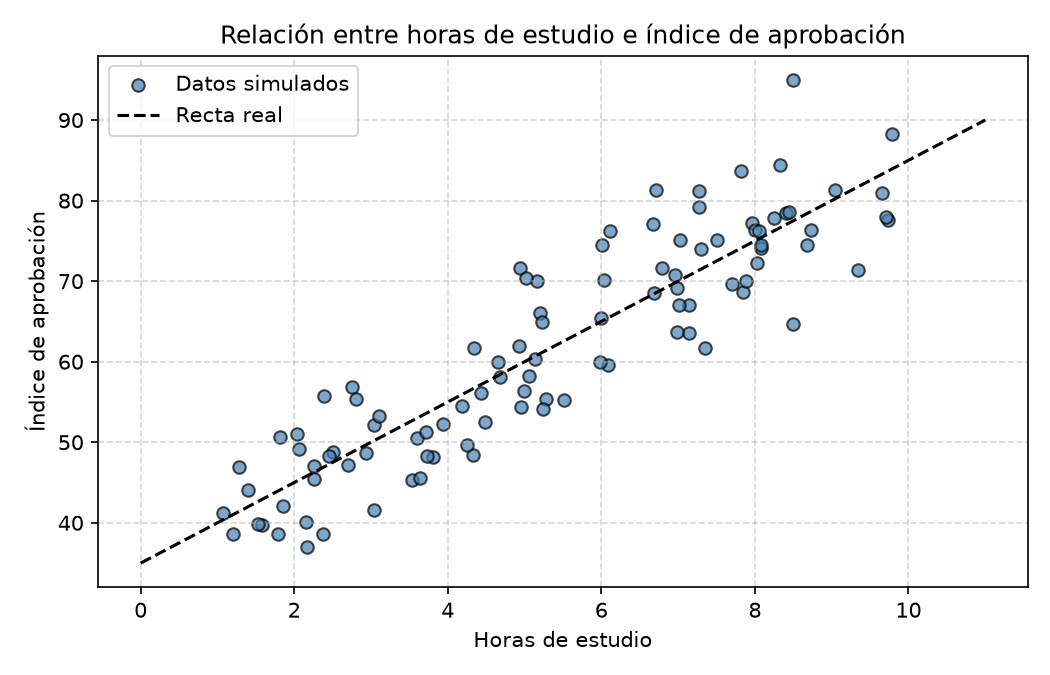
\includegraphics[width=0.7\textwidth]{img/datos_simulados.png}
\caption{Datos simulados de horas de estudio e índice de aprobación, con la recta real que los generó.}
\label{fig:datos}
\end{figure}

\subsection{Tarea 2: Modelo bayesiano de regresión lineal}

El Código~\ref{cod:t2} define el modelo de la sección anterior con PyMC y lo ajusta con cuatro cadenas de 2\,000 muestras cada una, después de 1\,000 pasos de calentamiento (8\,000 muestras posteriores). La función \texttt{modelo\_normal()} recibe los datos para poder reutilizarse en la extensión. Se genera además la Figura~\ref{fig:posterior}, con las trazas de las cadenas y la distribución posterior de cada parámetro, y la Figura~\ref{fig:regresion}, con la recta de regresión y su incertidumbre.

\begin{codigo}[label=cod:t2]{Tarea 2: modelo bayesiano de regresión lineal}
# indice_i ~ Normal(alfa + beta * horas_i, sigma)
# Priors débilmente informativos, a la escala del problema (índice de 0 a 100)
def modelo_normal(x, y):
    with pm.Model() as modelo:
        alfa = pm.Normal('alfa', mu=50, sigma=30)      # índice esperado con 0 horas
        beta = pm.Normal('beta', mu=0, sigma=10)       # puntos ganados por hora de estudio
        sigma = pm.HalfNormal('sigma', sigma=10)       # desviación del ruido
        mu = alfa + beta * x
        pm.Normal('y_obs', mu=mu, sigma=sigma, observed=y)
    return modelo


modelo = modelo_normal(datos['horas'].to_numpy(), datos['indice'].to_numpy())
with modelo:
    idata = pm.sample(2000, tune=1000, chains=4, random_seed=SEMILLA, progressbar=False)

print("\n=== Tarea 2: resumen de la distribución posterior ===")
resumen = az.summary(idata, var_names=['alfa', 'beta', 'sigma'], round_to=3)
print(resumen.to_string())
n_div = int(idata.sample_stats['diverging'].values.sum())
print(f"Divergencias: {n_div}")
reales = {'alfa': ALFA_REAL, 'beta': BETA_REAL, 'sigma': SIGMA_REAL}
for v, real in reales.items():
    m = muestras(idata, v)
    lo, hi = np.percentile(m, [3, 97])
    print(f"{v:<5} real = {real:<5} intervalo 94 %: [{lo:.2f}, {hi:.2f}]  contiene el real: {lo <= real <= hi}")

# Trazas por cadena y distribuciones posteriores
fig, ejes = plt.subplots(3, 2, figsize=(11, 8))
for fila, v in enumerate(('alfa', 'beta', 'sigma')):
    arr = idata.posterior[v].values  # (cadenas, pasos)
    for c in range(arr.shape[0]):
        ejes[fila, 0].plot(arr[c], linewidth=0.5, alpha=0.7)
    ejes[fila, 0].set_ylabel(v)
    ejes[fila, 1].hist(arr.reshape(-1), bins=50, density=True, color='skyblue', edgecolor='white')
    ejes[fila, 1].axvline(reales[v], color='k', linestyle='--', label='Valor real')
    ejes[fila, 1].set_xlabel(v)
    ejes[fila, 1].grid(linestyle='--', alpha=0.5)
ejes[0, 0].set_title('Trazas (4 cadenas)')
ejes[0, 1].set_title('Distribución posterior')
ejes[0, 1].legend()
ejes[2, 0].set_xlabel('Paso')
guardar('posterior.png')

# Recta de regresión con incertidumbre: 100 rectas posteriores y banda del 94 %
alfa_m, beta_m = muestras(idata, 'alfa'), muestras(idata, 'beta')
rectas = alfa_m[:, None] + beta_m[:, None] * xs[None, :]
banda = np.percentile(rectas, [3, 97], axis=0)
fig, ax = plt.subplots(figsize=(7, 4.5))
ax.scatter(datos['horas'], datos['indice'], color='steelblue', edgecolor='black', alpha=0.7,
           label='Datos', zorder=3)
for i in rng.choice(len(alfa_m), 100, replace=False):
    ax.plot(xs, rectas[i], color='gray', alpha=0.15, linewidth=0.8)
ax.fill_between(xs, banda[0], banda[1], color='orange', alpha=0.3, label='Banda de credibilidad 94 %')
ax.plot(xs, rectas.mean(axis=0), color='darkorange', linewidth=2, label='Recta posterior media')
ax.plot(xs, ALFA_REAL + BETA_REAL * xs, 'k--', linewidth=1.5, label='Recta real')
ax.set_xlabel('Horas de estudio')
ax.set_ylabel('Índice de aprobación')
ax.set_title('Regresión lineal bayesiana')
ax.legend()
ax.grid(linestyle='--', alpha=0.5)
guardar('regresion_posterior.png')
\end{codigo}

\begin{consola}[label=out:t2]{Ejecución de \texttt{act13.py}: Tarea 2}
=== Tarea 2: resumen de la distribución posterior ===
         mean     sd  eti89_lb  eti89_ub  ess_bulk  ess_tail  r_hat  mcse_mean  mcse_sd
alfa   34.725  1.460    32.354    37.083  3558.182  3658.571  1.001      0.024    0.019
beta    5.040  0.246     4.646     5.438  3573.979  3727.516  1.001      0.004    0.003
sigma   5.998  0.440     5.340     6.740  4040.085  3973.559  1.000      0.007    0.006
Divergencias: 0
alfa  real = 35.0  intervalo 94 %: [31.93, 37.44]  contiene el real: True
beta  real = 5.0   intervalo 94 %: [4.58, 5.50]  contiene el real: True
sigma real = 6.0   intervalo 94 %: [5.24, 6.91]  contiene el real: True
\end{consola}

El muestreo es confiable: $\hat{R}$ vale como máximo 1.001, el tamaño efectivo de muestra supera 3\,500 en los tres parámetros y no hubo divergencias. Las trazas de las cuatro cadenas se mezclan sin tendencias (Figura~\ref{fig:posterior}). Las medias posteriores son $\alpha = 34.73$, $\beta = 5.04$ y $\sigma = 6.00$, muy cercanas a los valores reales (35, 5 y 6), y los tres intervalos de credibilidad del 94\,\% contienen el valor real. La tabla de \texttt{az.summary} muestra por omisión intervalos del 89\,\%, y los del 94\,\% se calcularon aparte con percentiles. En términos del problema, cada hora adicional de estudio aumenta el índice en unos 5 puntos, con una incertidumbre de $\pm 0.25$ (una desviación estándar).

\begin{figure}[htbp]
\centering
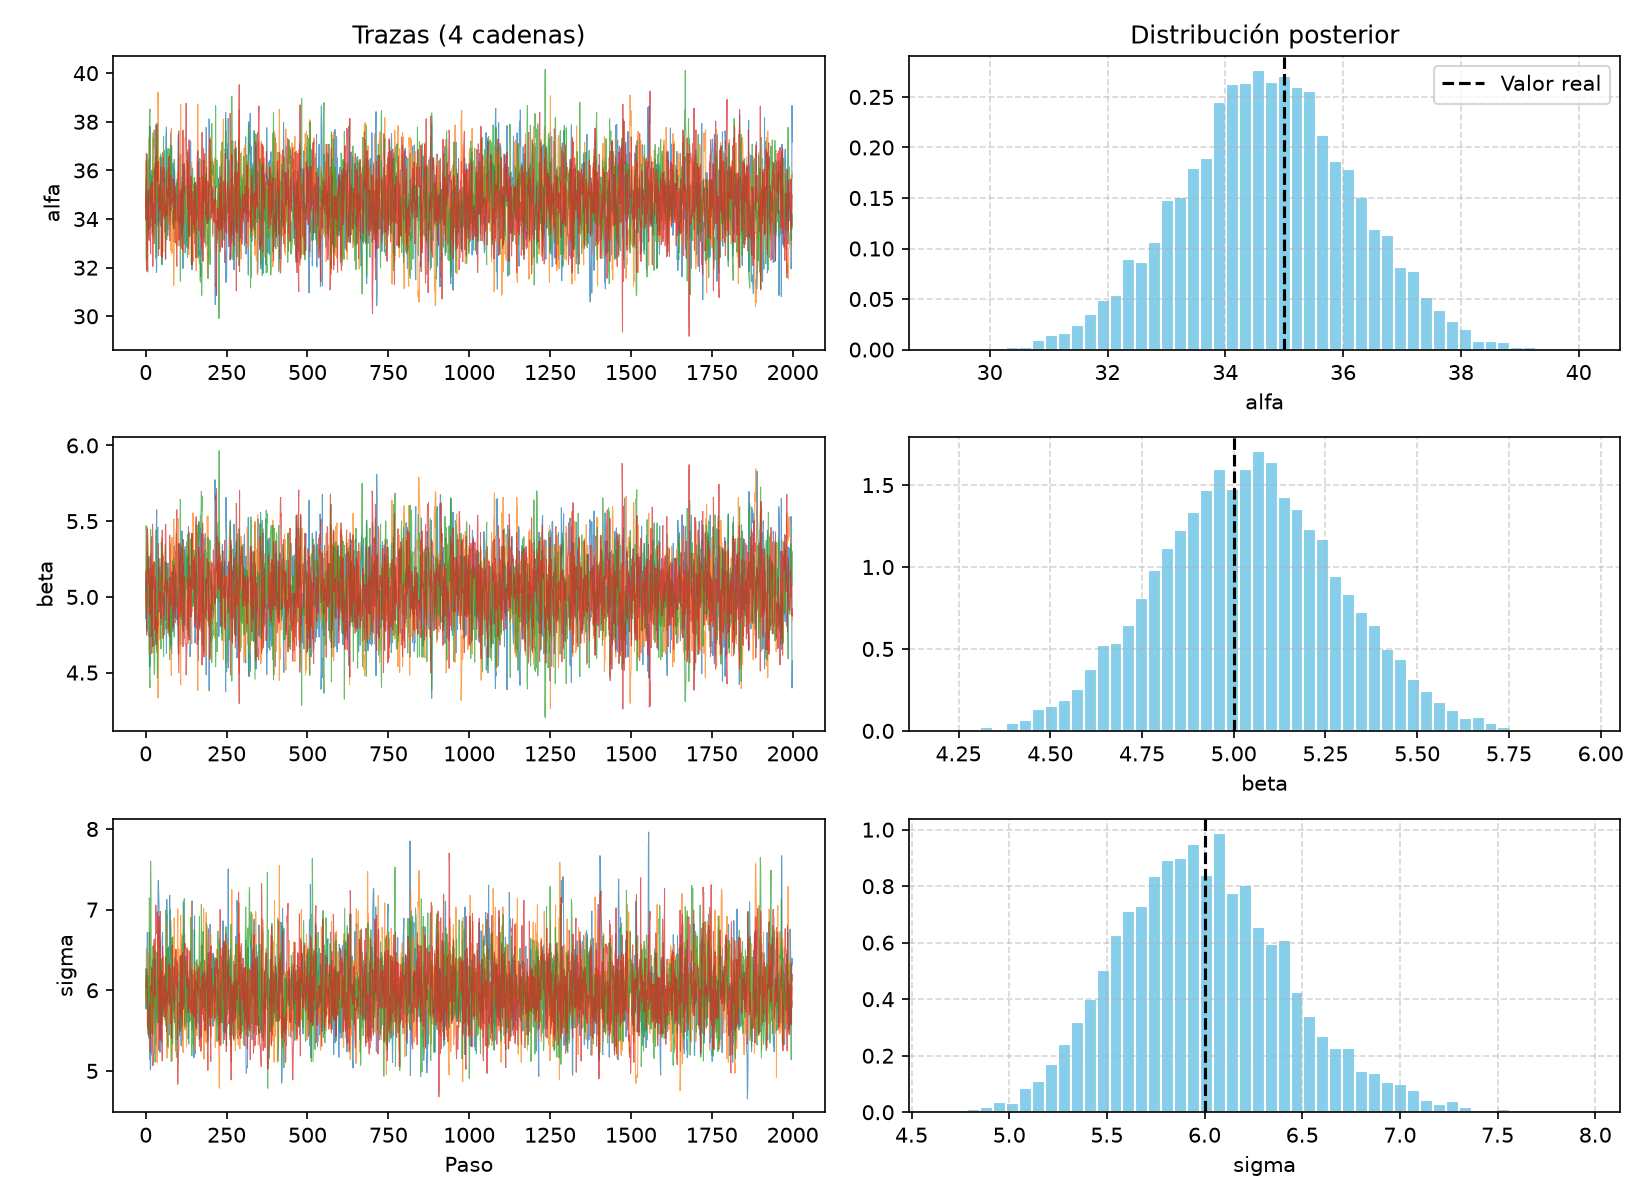
\includegraphics[width=0.9\textwidth]{img/posterior.png}
\caption{Trazas de las cuatro cadenas (izquierda) y distribución posterior de cada parámetro (derecha); la línea punteada es el valor real.}
\label{fig:posterior}
\end{figure}

\begin{figure}[htbp]
\centering
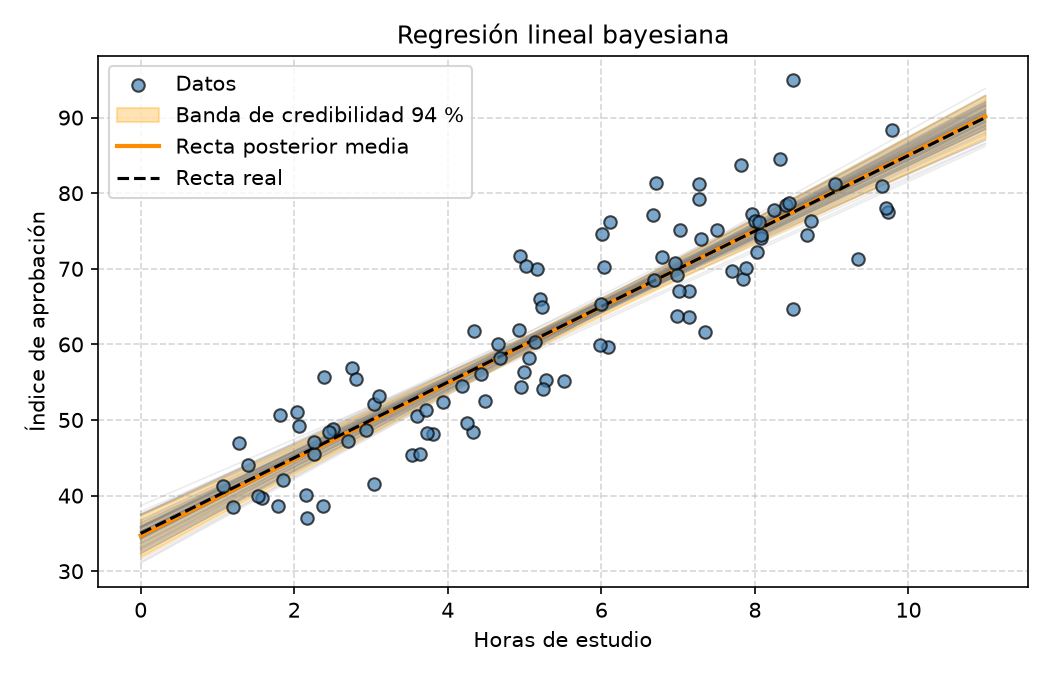
\includegraphics[width=0.7\textwidth]{img/regresion_posterior.png}
\caption{Regresión lineal bayesiana: 100 rectas tomadas de la posterior, banda de credibilidad del 94\,\% para la recta y recta real.}
\label{fig:regresion}
\end{figure}

La banda de la Figura~\ref{fig:regresion} es más ancha en los extremos de las horas que en el centro, porque ahí hay menos datos que fijen la recta. Esa banda es la incertidumbre sobre la recta; la incertidumbre sobre un estudiante concreto es mayor, porque incluye el ruido $\sigma$, y se evalúa en la tarea siguiente.

\subsection{Tarea 3: Posterior Predictive Check}

El Código~\ref{cod:t3} genera con \texttt{pm.sample\_posterior\_predictive()} un conjunto de 100 datos por cada una de las 8\,000 muestras posteriores. Con ellos se hacen tres comprobaciones (Figura~\ref{fig:ppc}): la densidad de los datos observados frente a la de los simulados, un estadístico (aquí la curtosis de los residuos) frente a su distribución simulada, y el intervalo predictivo del 94\,\% sobre los datos. Además, la función \texttt{estadisticos\_ppc()} calcula el valor $p$ bayesiano de la media, la desviación estándar, el mínimo, el máximo y la curtosis de los residuos de una recta de mínimos cuadrados (que mide si el ruido tiene colas más pesadas que las de una normal). Las mismas funciones se usan después en la extensión.

\begin{codigo}[label=cod:t3]{Tarea 3: Posterior Predictive Check}
# Se simulan conjuntos de datos nuevos con parámetros tomados de la posterior. Si el
# modelo es adecuado, los datos observados deben verse como uno más de los simulados.
def ppc(modelo, idata):
    with modelo:
        pm.sample_posterior_predictive(idata, extend_inferencedata=True, random_seed=SEMILLA,
                                       progressbar=False)
    return idata.posterior_predictive['y_obs'].values.reshape(-1, n)  # (simulaciones, n)


def valor_p(sim, observado):
    """Valor p bayesiano: proporción de simulaciones con el estadístico >= al observado.
    Valores cerca de 0 o de 1 indican que el modelo no reproduce esa característica."""
    return float(np.mean(sim >= observado))


# Matriz que convierte un conjunto de datos y en los residuos de la recta de mínimos cuadrados
# contra las horas (x fijo). Permite medir la forma del ruido alrededor de la recta.
X_DISENO = np.column_stack([np.ones(n), datos['horas'].to_numpy()])
M_RESIDUOS = np.eye(n) - X_DISENO @ np.linalg.solve(X_DISENO.T @ X_DISENO, X_DISENO.T)


def curtosis_res(a, axis=None):
    """Curtosis en exceso de los residuos de una recta MCO ajustada a cada conjunto de datos.
    Vale cerca de 0 si el ruido es normal y es alta si hay valores atípicos."""
    return stats.kurtosis(np.asarray(a) @ M_RESIDUOS.T, axis=-1)


ESTADISTICOS = {'media': np.mean, 'desv. estándar': np.std, 'mínimo': np.min, 'máximo': np.max,
                'curtosis de residuos': curtosis_res}


def estadisticos_ppc(sim, y):
    """Valor observado, media simulada y valor p de cada estadístico."""
    filas = {}
    for nombre, f in ESTADISTICOS.items():
        s = f(sim, axis=1)
        filas[nombre] = {'observado': f(y), 'simulado (media)': s.mean(), 'valor p': valor_p(s, f(y))}
    return pd.DataFrame(filas).T


def graficar_ppc(sim, x, y, nombre_archivo, titulo):
    """Tres paneles: densidades simuladas contra la observada, curtosis de residuos y banda predictiva."""
    fig, (ax1, ax2, ax3) = plt.subplots(1, 3, figsize=(15, 4.5))
    # (1) Densidad de 100 conjuntos simulados contra la observada
    mallas = np.linspace(y.min() - 30, y.max() + 30, 200)  # acotada: la t simula valores extremos
    for i in np.random.default_rng(SEMILLA).choice(len(sim), 100, replace=False):
        ax1.plot(mallas, stats.gaussian_kde(sim[i])(mallas), color='tab:blue', alpha=0.15)
    ax1.plot(mallas, stats.gaussian_kde(y)(mallas), color='k', linewidth=2.5, label='Observado')
    ax1.plot([], [], color='tab:blue', label='Simulados (PPC)')
    ax1.set_xlabel('Índice de aprobación')
    ax1.set_ylabel('Densidad')
    ax1.set_title('Densidades observada y simuladas')
    ax1.legend()
    ax1.grid(linestyle='--', alpha=0.5)
    # (2) Curtosis de los residuos: colas del ruido alrededor de la recta
    s_k = curtosis_res(sim)
    obs_k = float(curtosis_res(y))
    tope = max(np.percentile(s_k, 99), obs_k) * 1.1
    ax2.hist(s_k[s_k <= tope], bins=50, density=True, color='tab:green', alpha=0.6, label='Simulado')
    ax2.axvline(obs_k, color='k', linewidth=2.5, linestyle='--', label='Observado')
    ax2.set_xlabel('Curtosis de los residuos')
    ax2.set_ylabel('Densidad')
    ax2.set_title('Colas del ruido (valores > percentil 99 omitidos)')
    ax2.legend()
    ax2.grid(linestyle='--', alpha=0.5)
    # (3) Banda predictiva del 94 % contra los datos
    orden = np.argsort(x)
    lo, hi = np.percentile(sim, [3, 97], axis=0)
    ax3.fill_between(x[orden], lo[orden], hi[orden], color='orange', alpha=0.3,
                     label='Intervalo predictivo 94 %')
    ax3.scatter(x, y, color='steelblue', edgecolor='black', alpha=0.7, label='Datos')
    ax3.set_ylim(y.min() - 30, y.max() + 30)
    ax3.set_xlabel('Horas de estudio')
    ax3.set_title('Banda predictiva')
    ax3.legend()
    ax3.grid(linestyle='--', alpha=0.5)
    fig.suptitle(titulo)
    guardar(nombre_archivo)


x_obs, y_obs = datos['horas'].to_numpy(), datos['indice'].to_numpy()
sim = ppc(modelo, idata)
tabla_ppc = estadisticos_ppc(sim, y_obs)
cobertura = float(np.mean((y_obs >= np.percentile(sim, 3, axis=0)) & (y_obs <= np.percentile(sim, 97, axis=0))))

print("\n=== Tarea 3: Posterior Predictive Check ===")
print(f"Simulaciones: {sim.shape[0]} conjuntos de {sim.shape[1]} datos")
print(tabla_ppc.round(3).to_string())
print(f"Cobertura del intervalo predictivo 94 %: {cobertura:.0%} de los datos observados")
graficar_ppc(sim, x_obs, y_obs, 'ppc_normal.png', 'PPC del modelo normal')
\end{codigo}

\begin{consola}[label=out:t3]{Ejecución de \texttt{act13.py}: Tarea 3}
=== Tarea 3: Posterior Predictive Check ===
Simulaciones: 8000 conjuntos de 100 datos
                      observado  simulado (media)  valor p
media                    61.818            61.838    0.513
desv. estándar           13.700            13.703    0.490
mínimo                   37.022            32.314    0.074
máximo                   94.954            91.431    0.168
curtosis de residuos     -0.210            -0.061    0.581
Cobertura del intervalo predictivo 94 %: 96% de los datos observados
\end{consola}

\begin{figure}[htbp]
\centering
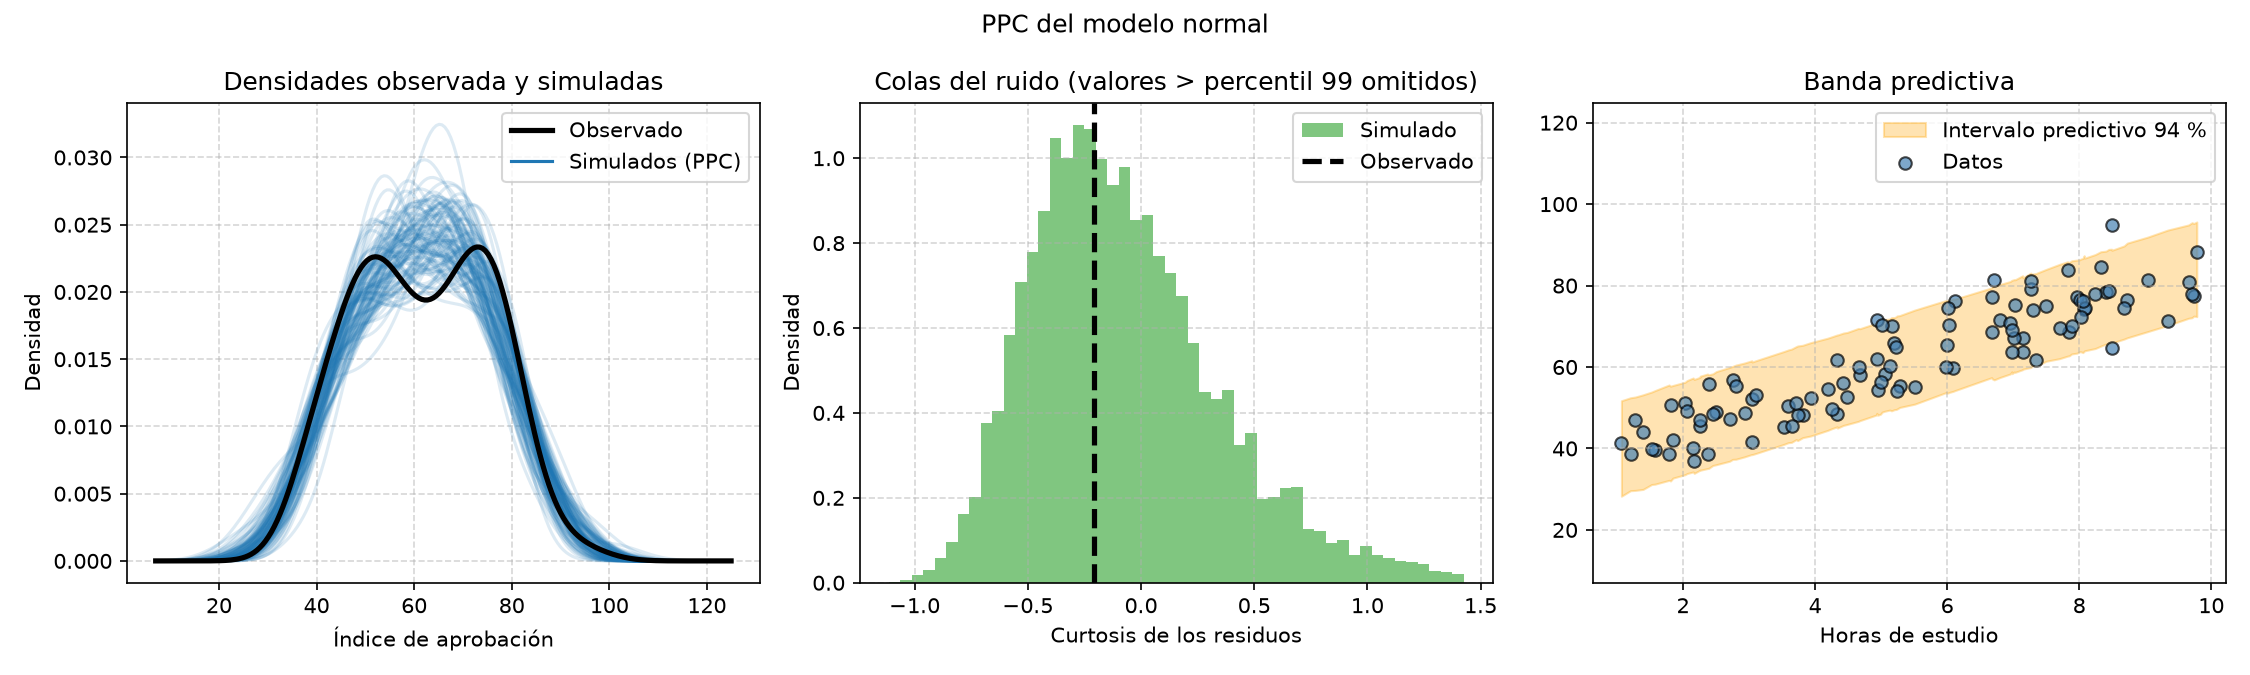
\includegraphics[width=\textwidth]{img/ppc_normal.png}
\caption{PPC del modelo normal. Izquierda: densidad observada (negro) y 100 simuladas. Centro: curtosis de los residuos simulada y observada. Derecha: intervalo predictivo del 94\,\%.}
\label{fig:ppc}
\end{figure}

El modelo se ajusta bien a los datos:
\begin{itemize}
    \item \textbf{Densidades.} La curva observada queda dentro del conjunto de curvas simuladas. Su forma con dos jorobas no es una falla del modelo: viene de que las horas se simularon con distribución uniforme, y las simulaciones, que usan las mismas horas, producen formas parecidas.
    \item \textbf{Estadísticos.} Todos los valores $p$ son intermedios: 0.51 para la media, 0.49 para la desviación estándar, 0.58 para la curtosis de residuos, y 0.17 y 0.07 para el máximo y el mínimo. El mínimo es el más bajo, pero sigue por encima de 0.05 y la diferencia es pequeña (el mínimo simulado promedia 32.3 contra 37.0 observado), por lo que no se considera una falla.
    \item \textbf{Intervalo predictivo.} El intervalo del 94\,\% contiene al 96\,\% de los datos observados, lo esperado.
\end{itemize}

\subsection{Extensión: datos atípicos y modelo robusto}

El documento fuente indica que, si hay valores atípicos que violan el supuesto de normalidad, se puede sustituir la normal por una t de Student \parencite{tecnm2026_documento_fuente}. Para verlo, se contaminaron los datos: seis estudiantes con muchas horas de estudio (de 7.3 a 9.7) tienen un índice entre 5 y 25 puntos, en lugar de los 70 o más que les correspondían (Código~\ref{cod:ext}). Se ajustaron dos modelos: el normal anterior y uno igual pero con verosimilitud t de Student, con $\nu \sim \mathrm{Exponencial}(1/30)$ como en el documento fuente.

\begin{codigo}[label=cod:ext]{Extensión: datos atípicos y modelo robusto}
# Se contaminan 6 estudiantes que estudiaron mucho pero obtuvieron un índice muy bajo.
# El modelo normal no los espera; el PPC debe delatarlo y la t de Student corregirlo.
idx_atipicos = np.argsort(x_obs)[-30:][np.random.default_rng(SEMILLA).choice(30, 6, replace=False)]
y_atip = y_obs.copy()
y_atip[idx_atipicos] = rng.uniform(5, 25, size=6)


def modelo_t(x, y):
    with pm.Model() as modelo:
        alfa = pm.Normal('alfa', mu=50, sigma=30)
        beta = pm.Normal('beta', mu=0, sigma=10)
        sigma = pm.HalfNormal('sigma', sigma=10)
        nu = pm.Exponential('nu', 1 / 30)              # grados de libertad de la t
        mu = alfa + beta * x
        pm.StudentT('y_obs', mu=mu, sigma=sigma, nu=nu, observed=y)
    return modelo


modelo_n2 = modelo_normal(x_obs, y_atip)
modelo_t2 = modelo_t(x_obs, y_atip)
with modelo_n2:
    idata_n2 = pm.sample(2000, tune=1000, chains=4, random_seed=SEMILLA, progressbar=False)
with modelo_t2:
    idata_t2 = pm.sample(2000, tune=1000, chains=4, random_seed=SEMILLA, progressbar=False)
sim_n2, sim_t2 = ppc(modelo_n2, idata_n2), ppc(modelo_t2, idata_t2)

print("\n=== Extensión: datos con 6 atípicos ===")
print(f"Atípicos en las posiciones de horas: {np.round(np.sort(x_obs[idx_atipicos]), 2)}")
for nombre, idt in (('Normal', idata_n2), ('t de Student', idata_t2)):
    print(f"\n{nombre}:")
    cols = ['alfa', 'beta', 'sigma'] + (['nu'] if nombre != 'Normal' else [])
    print(az.summary(idt, var_names=cols, round_to=3)[['mean', 'sd', 'r_hat']].to_string())
print("\nPPC del modelo normal con atípicos:")
print(estadisticos_ppc(sim_n2, y_atip).round(3).to_string())
print("\nPPC del modelo t de Student con atípicos:")
print(estadisticos_ppc(sim_t2, y_atip).round(3).to_string())
graficar_ppc(sim_n2, x_obs, y_atip, 'ppc_normal_atipicos.png', 'PPC del modelo normal con atípicos')
graficar_ppc(sim_t2, x_obs, y_atip, 'ppc_t_atipicos.png', 'PPC del modelo t de Student con atípicos')

# Efecto de los atípicos sobre la pendiente
fig, ax = plt.subplots(figsize=(7, 4))
ax.hist(muestras(idata_n2, 'beta'), bins=50, density=True, alpha=0.6, label='Normal', color='tab:red')
ax.hist(muestras(idata_t2, 'beta'), bins=50, density=True, alpha=0.6, label='t de Student',
        color='tab:blue')
ax.axvline(BETA_REAL, color='k', linestyle='--', label='Valor real')
ax.set_xlabel('beta (puntos por hora de estudio)')
ax.set_ylabel('Densidad')
ax.set_title('Pendiente posterior con datos atípicos')
ax.legend()
ax.grid(linestyle='--', alpha=0.5)
guardar('beta_atipicos.png')
\end{codigo}

\begin{consola}[label=out:ext]{Ejecución de \texttt{act13.py}: extensión}
=== Extensión: datos con 6 atípicos ===
Atípicos en las posiciones de horas: [7.28 8.03 8.33 8.49 9.34 9.74]

Normal:
         mean     sd  r_hat
alfa   41.147  3.620  1.001
beta    3.196  0.615  1.001
sigma  15.123  1.078  1.000

t de Student:
         mean     sd  r_hat
alfa   34.149  1.434  1.001
beta    5.040  0.246  1.002
sigma   4.682  0.619  1.001
nu      1.747  0.365  1.001

PPC del modelo normal con atípicos:
                      observado  simulado (media)  valor p
media                    58.303            58.336    0.509
desv. estándar           16.954            16.964    0.486
mínimo                   12.702            15.797    0.684
máximo                   94.954           100.685    0.763
curtosis de residuos      6.218            -0.061    0.000

PPC del modelo t de Student con atípicos:
                      observado  simulado (media)  valor p
media                    58.303            61.203    0.918
desv. estándar           16.954            29.659    0.614
mínimo                   12.702           -68.695    0.411
máximo                   94.954           189.518    0.855
curtosis de residuos      6.218            22.999    0.760
\end{consola}

\begin{table}[htbp]
\centering
\caption{Parámetros reales y medias posteriores con 6 valores atípicos.}
\label{tab:ext}
\small
\begin{tabular}{lccc}
\hline
\textbf{Parámetro} & \textbf{Real} & \textbf{Modelo normal} & \textbf{Modelo t de Student} \\
\hline
$\alpha$ & 35 & 41.15 & 34.15 \\
$\beta$ & 5 & 3.20 & 5.04 \\
$\sigma$ & 6 & 15.12 & 4.68 \\
$\nu$ & --- & --- & 1.75 \\
\hline
\end{tabular}
\end{table}

\begin{figure}[htbp]
\centering
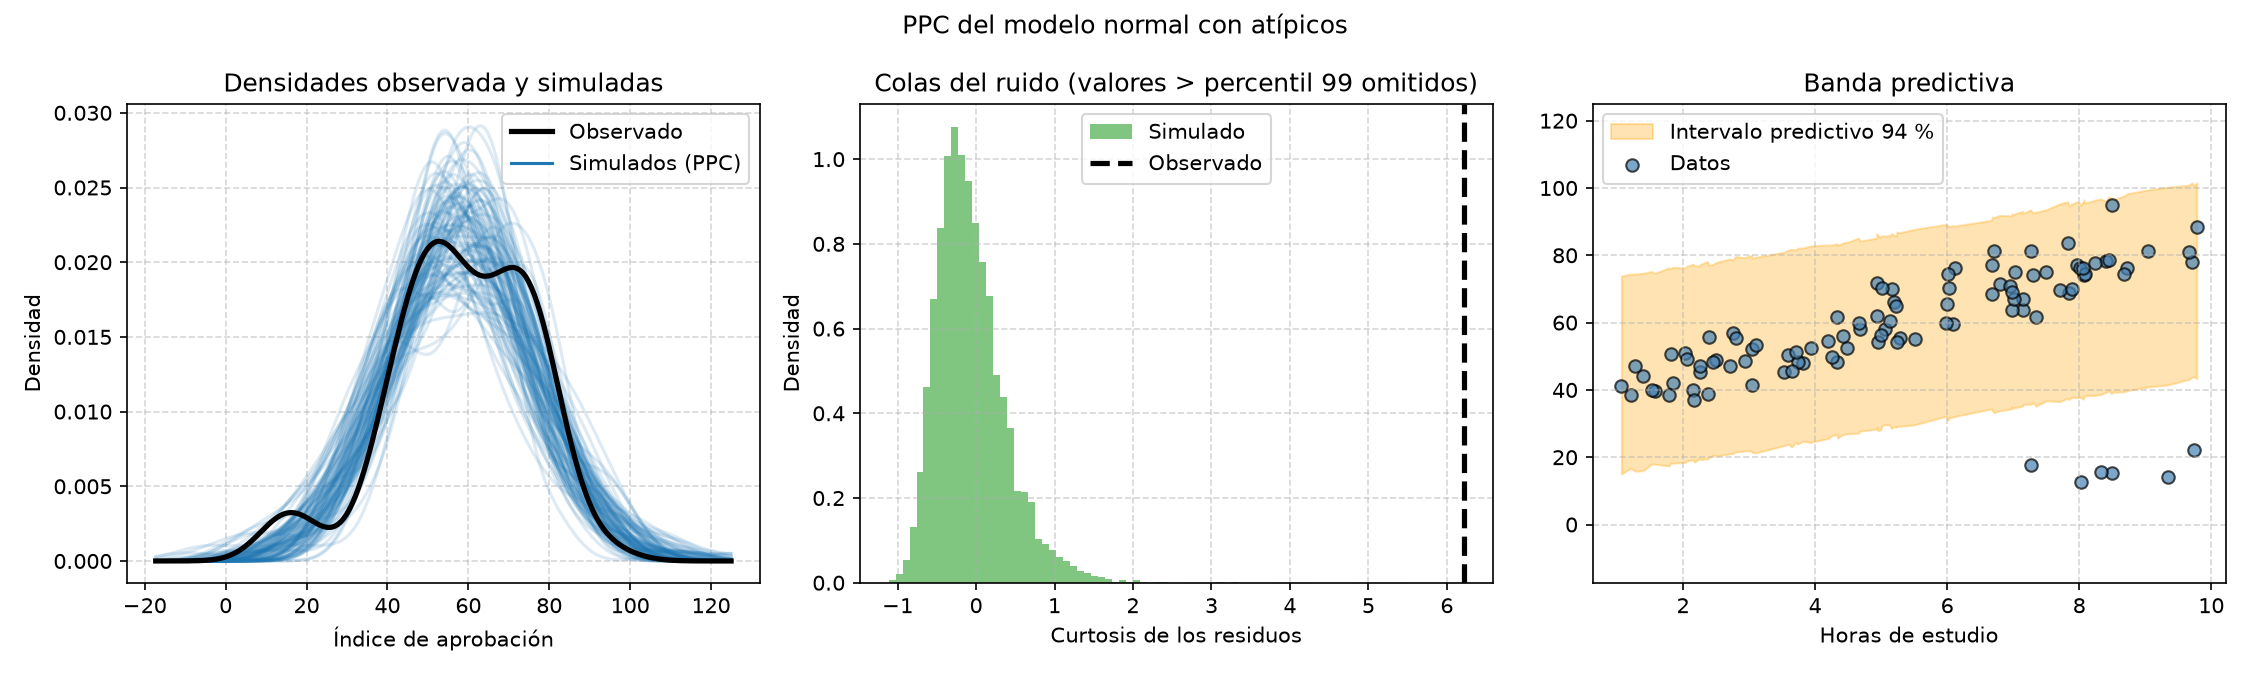
\includegraphics[width=\textwidth]{img/ppc_normal_atipicos.png}
\caption{PPC del modelo normal con valores atípicos.}
\label{fig:ppc-normal-atip}
\end{figure}

\begin{figure}[htbp]
\centering
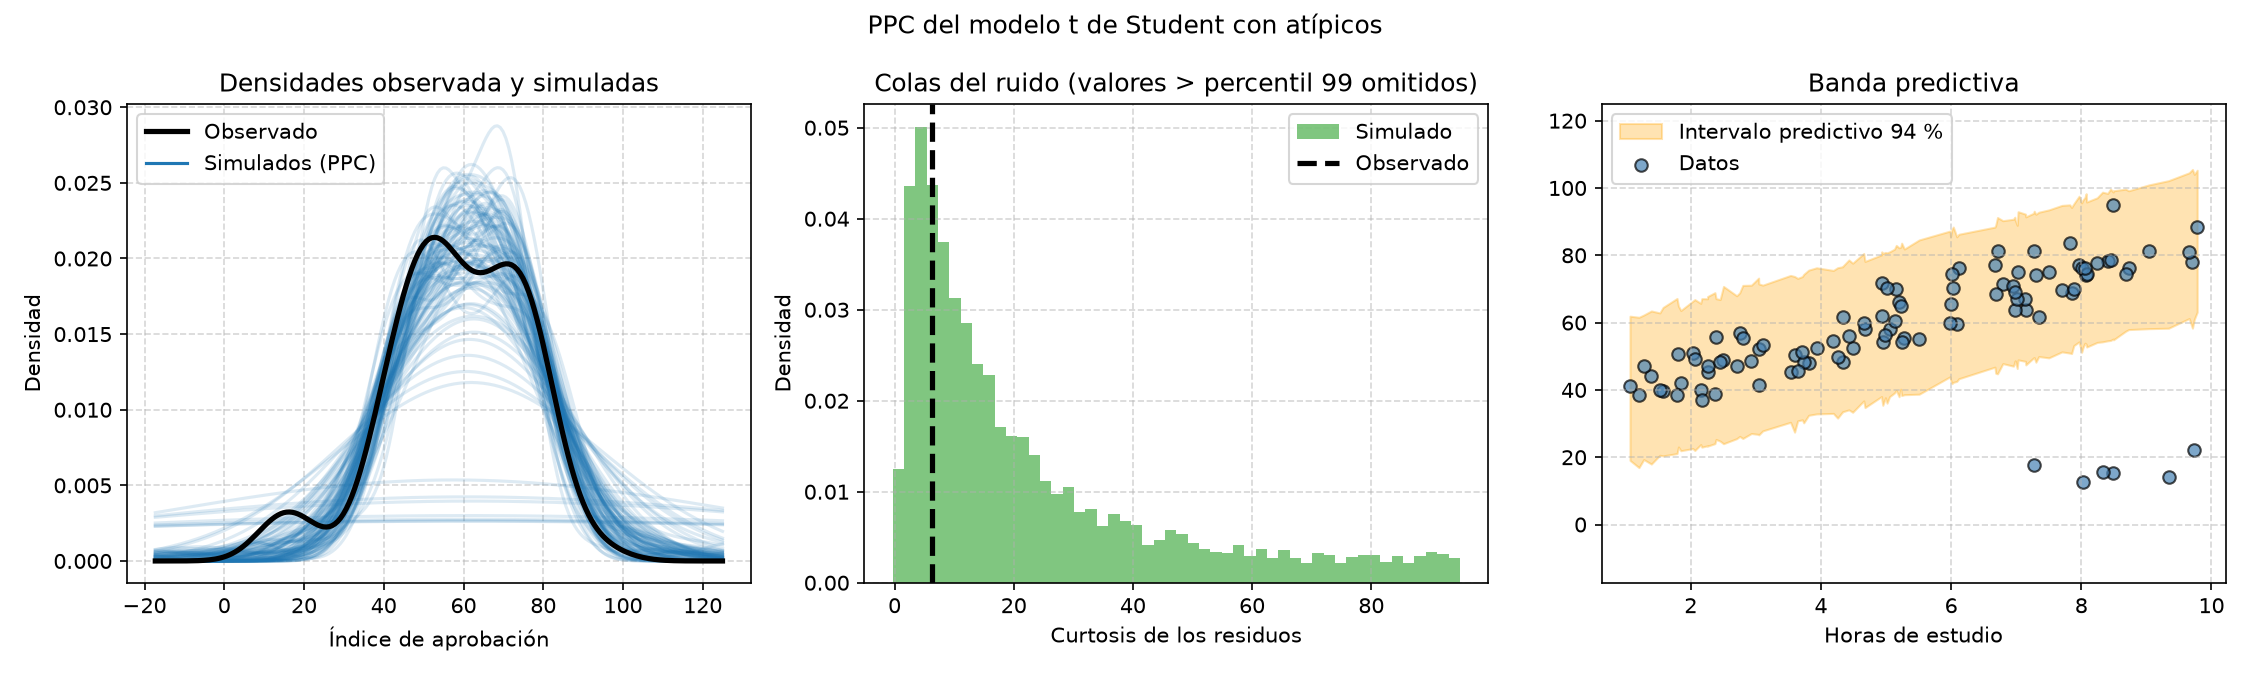
\includegraphics[width=\textwidth]{img/ppc_t_atipicos.png}
\caption{PPC del modelo t de Student con valores atípicos.}
\label{fig:ppc-t-atip}
\end{figure}

\begin{figure}[htbp]
\centering
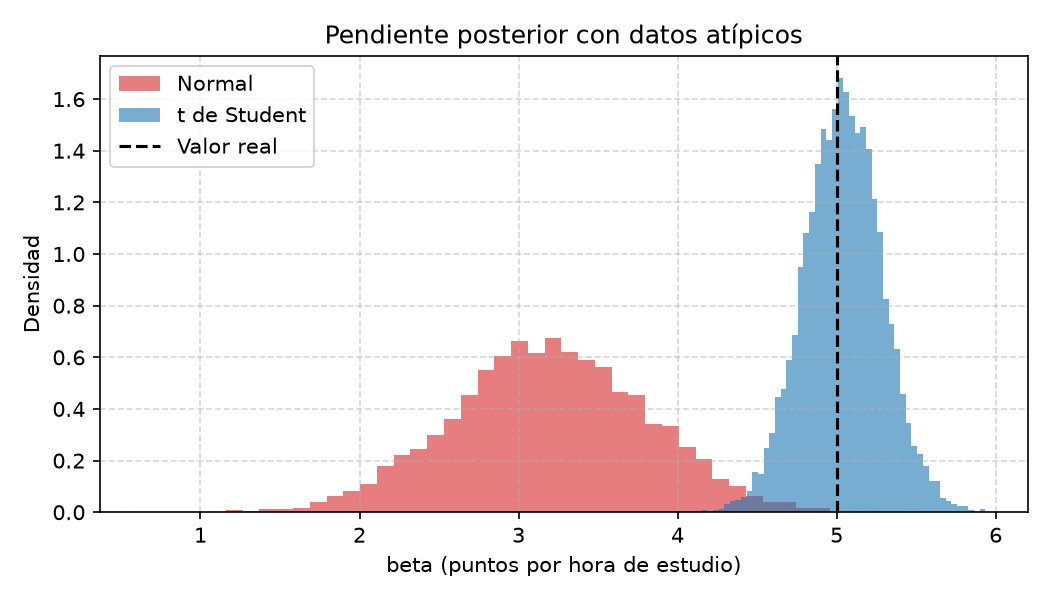
\includegraphics[width=0.6\textwidth]{img/beta_atipicos.png}
\caption{Distribución posterior de la pendiente con valores atípicos en los dos modelos.}
\label{fig:beta-atip}
\end{figure}

\begin{itemize}
    \item \textbf{El modelo normal se distorsiona.} Los seis atípicos desplazan la recta ($\beta = 3.20$ en vez de 5, con una posterior que ya no contiene el valor real, Figura~\ref{fig:beta-atip}) y multiplican por 2.5 la desviación ($\sigma = 15.1$ contra 6). Aun así, los seis atípicos quedan por debajo de la banda predictiva de la Figura~\ref{fig:ppc-normal-atip}, y la banda es demasiado holgada para los 94 datos restantes.
    \item \textbf{Qué detecta el PPC.} Los estadísticos globales no delatan el problema: la media, la desviación estándar, el mínimo y el máximo tienen valores $p$ intermedios (0.51, 0.49, 0.68 y 0.76), porque el modelo infló $\sigma$ hasta absorber los extremos. Lo que sí lo delata es la curtosis de los residuos: la observada es 6.22 y las simuladas casi nunca pasan de 2, con un valor $p$ de 0.000 (Figura~\ref{fig:ppc-normal-atip}, centro). Es decir, el modelo normal solo es capaz de producir ruido con colas ligeras y los datos tienen colas pesadas. Este estadístico se eligió después de comprobar que los demás no distinguían los modelos, por lo que es una prueba que se escogió con conocimiento de los datos; se justifica porque mide la característica que la normal no puede reproducir.
    \item \textbf{La t de Student corrige la estimación.} Recupera los parámetros ($\beta = 5.04$, $\sigma = 4.68$, $\alpha = 34.15$) y reproduce la curtosis observada (valor $p$ de 0.76), porque con $\nu = 1.75$ trata a los seis atípicos como colas de la distribución en vez de forzar la recta hacia ellos. Su $\sigma$ queda algo debajo del real (4.68 contra 6), pues parte de la dispersión se atribuye a las colas.
    \item \textbf{Pero tiene un costo.} Un $\nu$ tan pequeño equivale a colas casi tan pesadas como las de una Cauchy, y el modelo llega a simular índices imposibles: el mínimo simulado promedia $-69$ y el máximo 190, en un índice limitado de 0 a 100, y la desviación simulada (29.7) es mucho mayor que la observada (17.0). Los valores $p$ de estos estadísticos son intermedios (0.41 y 0.86) porque la distribución simulada es muy dispersa, no porque sean realistas. Se ve en la Figura~\ref{fig:ppc-t-atip} (izquierda), donde algunas curvas simuladas son casi planas. Un modelo de mezcla, que separe a la mayoría de los estudiantes del pequeño grupo atípico, o uno que tome en cuenta el límite del índice, sería más adecuado.
\end{itemize}

\section{Conclusiones}

Se construyó un modelo predictivo bayesiano completo con PyMC. Con datos simulados de una relación lineal entre horas de estudio e índice de aprobación, la distribución posterior recuperó los parámetros verdaderos: los intervalos de credibilidad del 94\,\% de $\alpha$, $\beta$ y $\sigma$ contienen los valores reales, y el muestreo fue confiable ($\hat{R} \le 1.001$, ESS superior a 3\,500 y sin divergencias). Con una media posterior de $\beta$ de 5.04, cada hora de estudio adicional sube el índice en unos 5 puntos, con una incertidumbre cuantificada.

El Posterior Predictive Check mostró que, con datos generados por un proceso normal, el modelo normal es adecuado: las densidades simuladas envuelven a la observada, los valores $p$ de los estadísticos fueron intermedios (el menor, 0.07, para el mínimo) y el intervalo predictivo del 94\,\% cubrió al 96\,\% de los datos. Esto es de esperarse, pues los datos se generaron con el mismo modelo con el que se ajustaron, y hay que recordar que el PPC usa los datos de ajuste, por lo que es una prueba permisiva.

En la extensión, el PPC permitió detectar que el supuesto de normalidad no se cumple cuando hay valores atípicos, aunque no con cualquier estadístico: la media, la desviación, el mínimo y el máximo no lo detectaron, porque el modelo infló $\sigma$ para absorber los atípicos, y fue la curtosis de los residuos la que lo evidenció. Esto indica que conviene revisar un PPC con estadísticos distintos y elegirlos según el supuesto que se quiere verificar. Sustituir la normal por la t de Student corrigió las estimaciones ($\beta$ pasó de 3.20 a 5.04), pero con $\nu = 1.75$ el modelo produce predicciones fuera del rango posible del índice, por lo que no es una solución completa. La conclusión general es que verificar los supuestos, ajustar el modelo y volver a verificar es un ciclo, y que un modelo que corrige un problema puede introducir otro que solo se ve al volver a evaluarlo.

\referencias

\end{document}
